\documentclass[11pt]{article}
\usepackage[margin=1in]{geometry}
\usepackage{graphicx}
\usepackage{booktabs}
\usepackage{amsmath}
\usepackage{amssymb}
\usepackage{float}
\usepackage{hyperref}
\usepackage{caption}
\usepackage{array}
\usepackage{pgffor}
\usepackage{listings}
\usepackage{placeins}
\usepackage{setspace}
\usepackage{titlesec}
\usepackage{hyperref}

\titleformat{\paragraph}[block]{\normalfont\normalsize\bfseries}{}{0pt}{}

\lstset{
  basicstyle=\ttfamily\small,
  columns=fullflexible,
  keepspaces=true,
  frame=single,
  breaklines=true,
  showstringspaces=false
}

\setstretch{1.1}
\setlength{\parskip}{0.45em}
\setlength{\parindent}{0pt}
\setlength{\textfloatsep}{12pt plus 2pt minus 4pt}
\setlength{\floatsep}{10pt plus 2pt minus 4pt}
\setlength{\intextsep}{10pt plus 2pt minus 4pt}
\titlespacing*{\subsection}{0pt}{1.5em}{0.9em}
\titlespacing*{\subsubsection}{0pt}{1.3em}{0.8em}
\titlespacing*{\paragraph}{0pt}{1.1em}{0.5em}

\title{Title}
\author{Numerical Analysis Project}
\date{March 9, 2026}

\newcommand{\artifactinput}[1]{%
  \IfFileExists{#1}{\input{#1}}{\textit{Missing artifact: #1}}
}

\newcommand{\artifactfigure}[3]{%
  \IfFileExists{#1}{%
    \begin{figure}[!htbp]
    \centering
    \includegraphics[width=#2\linewidth]{#1}
    \caption{#3}
    \end{figure}
  }{%
    \paragraph{Missing artifact} #1
  }%
}

% Toggle to include the full appendix wall figures (large output).
\newif\ifincludeappendixwalls
\includeappendixwallstrue

\begin{document}
\maketitle

\begin{abstract}

\end{abstract}

\section{Introduction}
Image data is common in many computing applications, such as medical diagnostics, remote sensing, and multimedia communication. In many of these image-based computing tasks, the manipulation and analysis of images can be achieved by solving a system of linear equations, as defined by the model, the image, or the process. In this context, the linear equation can be expressed as a matrix, which can be either dense or sparse, depending on the image data and the model. Gaussian elimination, LU decomposition, Gauss-Seidel method with relaxation, and hybrid Krylov subspace methods such as GMRES are some of the fundamental numerical analysis techniques that can be applied to compute the solution to the linear equation.

However, in real-world problems, image data is often subject to random perturbations such as noise, transmission error, compression artifacts, and storage corruption. Small perturbations in the data may cause significant effects on the computation results. This sensitivity is conceptually similar to the avalanche effect in cryptographic systems, where a small change in the input causes a significant change in the output. In image encryption studies, the robustness of the diffusion properties is exploited to enhance the avalanche effect, yet this phenomenon also causes severe error propagation on the corrupted encrypted images, which makes the recovery of the image difficult or impossible (Noura et al., 2017). This shows how small numerical perturbations may cause severe distortion in the image data.

Moreover, in the field of research on image encryption, the significance of robustness in the presence of differential modifications is stressed, while at the same time, the danger of over-sensitivity to such modifications is also pointed out (Alghamdi \& Munir, 2024). Even though the major concern in research on image encryption is centered on security issues, the research shows that computational studies face a fundamental problem which requires assessment of image processing tasks to be evaluated for both performance and their ability to withstand noisy or damaged conditions. Similarly, in numerical linear algebra, any modification in the elements of a matrix could affect the overall behavior of the elimination process.

These considerations highlight the importance of systematically comparing how different numerical solvers respond to stochastic corruption in image-derived linear systems. In particular, the current study aims to test the baseline stability of the numerical solver that is based on the algorithm of Gaussian Elimination with Partial Pivoting, the block-reusability efficiency of the numerical solver that is based on the algorithm of LU Decomposition, the smoothing effects of the numerical solver that is based on the algorithm of Gauss-Seidel with Relaxation, and the robustness of the numerical solver that is based on the algorithm of Hybrid GMRES.


\section{Preliminaries}

In this section, the major concepts used in this research are discussed. These include the Hill cipher, dense and sparse matrices, and the four numerical solvers used in the research: Gauss-Elimination, LU Decomposition, Gauss-Seidel, and GMRES. It also defines the image quality metrics, Mean Square Error (MSE) and Peak Signal-to-Noise Ratio (PSNR), that serve as benchmarks for assessing solver performance under stochastic data corruption.

\subsection{Hill Cipher}

The Hill cipher is a classical polygraphic substitution cipher developed by Lester S. Hill in 1929. The Hill cipher was based on the principles of linear algebra. It is different from other substitution ciphers like the Caesar cipher, which was based on single-character substitution. In the Hill cipher, blocks of characters are considered to be vectors and are multiplied by a matrix to perform substitution.

In mathematical form, encryption is defined as:
$$ \mathbf{C} = \mathbf{K} \cdot \mathbf{P} \pmod{m} $$
Where:
\begin{itemize}
    \item $\mathbf{P}$ is the plaintext vector,
    \item $\mathbf{K}$ is the invertible key matrix,
    \item $\mathbf{C}$ is the ciphertext vector, and
    \item $m$ is the modulus, which is commonly 26 for text and 256 for 8-bit grayscale images.
\end{itemize}

A Hill cipher is only valid if the key matrix $\mathbf{K}$ is invertible in $\mathbb{Z}_m$. This requires that the determinant of the matrix and the modulus are coprime:
$$ \gcd(\det(\mathbf{K}), m) = 1 $$

Decryption is performed using the inverse key matrix:
$$ \mathbf{P} = \mathbf{K}^{-1} \cdot \mathbf{C} \pmod{m} $$

When this is applied to a digital image, pixel value information is arranged in vectors or matrix blocks and encrypted using the same linear transformation principle. Due to the high redundancy of image information, which is caused by the high correlation of pixel information, the Hill Cipher adds a diffusion effect by mixing pixel value information in the matrix blocks, thus breaking the correlation of the pixel information. 

The decryption process is highly sensitive to numerical inaccuracies. Inaccurate information introduced to the ciphertext during transmission can affect the matrix inversion, leading to degradation of the image. This is relevant to the robustness of the solver when analyzing the effect of stochastic corruption.

\subsection{Numerical Solvers}

\subsubsection{Gaussian Elimination}
Gaussian elimination with backward substitution is an algorithm used to solve a system of $n$ linear equations in $n$ variables represented as $\mathbf{A}\mathbf{x}=\mathbf{b}$, where $\mathbf{A}$ is the coefficient matrix, $\mathbf{x}$ is the vector of variables, and $\mathbf{b}$ is the constant vector. The main goal of the Gaussian elimination algorithm is to transform the augmented matrix of the system into an equivalent upper triangular matrix form. This is achieved by a sequence of elimination operations on the variables of the system through three basic row operations that do not change the solution set of the system of equations:
\begin{itemize}
    \item \textbf{Scaling:} $(\lambda E_i) \rightarrow (E_i)$ where $\lambda \neq 0$.
    \item \textbf{Row replacement:} $(E_i + \lambda E_j) \rightarrow (E_i)$.
    \item \textbf{Row interchanging:} $(E_i) \leftrightarrow (E_j)$.
\end{itemize}

The Gaussian elimination algorithm has two main steps:
\begin{enumerate}
    \item \textbf{Elimination Phase:} The main goal of the elimination phase is to eliminate the elements below the main diagonal of the augmented matrix of the system through the application of the basic row operations. If the element in the $i$-th row and $i$-th column, i.e., $a_{ii}$, is zero, the rows $E_i$ and $E_j$ should be interchanged, where $E_i$ is the current row of the augmented matrix, and $E_j$ is the row in the augmented matrix such that the element in the $j$-th column of $E_j$ is not zero.
    \item \textbf{Backward Substitution Phase:} The system is reduced to upper triangular form, and the variables are then recovered in reverse order:
    \[
    x_n, \; x_{n-1}, \; \dots, \; x_1.
    \]
\end{enumerate}

The computational cost of the Gaussian elimination algorithm for a system of $n$ linear equations in $n$ variables is on the order of $\mathcal{O}(n^3)$ for multiplications/divisions as well as additions/subtractions.

\paragraph{Stability and Noise Sensitivity}
A key component of the experimental protocol is the Noise Injection stress test, where Gaussian White Noise is added to the encrypted blocks ($\mathbf{C}' = \mathbf{C} + \varepsilon$). 
\begin{itemize}
    \item \textbf{Rounding Errors:} As the computational cost of the Gaussian Elimination method is given by $\mathcal{O}(n^3)$, the rounding errors that occur during the elimination of 64 variables resulting from an $8 \times 8$ matrix can cause salt-and-pepper noise to be introduced in the reconstructed image if the key matrix is poorly conditioned.
    \item \textbf{Partial Pivoting:} To enhance the robustness of the system, the algorithm makes use of the Partial Pivoting method. By choosing the pivot with the maximum value during the scaling operation, the effects of the injected random noise are reduced to ensure the accuracy of the Baseline recovery for comparison with the Gauss-Seidel method.
\end{itemize}

\subsubsection{LU Decomposition}
The LU factorization is a particularly useful factorization of a matrix $\mathbf{A}$ where $\mathbf{A}=\mathbf{L}\mathbf{U}$:
\begin{itemize}
    \item $\mathbf{L}$ is a lower triangular matrix.
    \item $\mathbf{U}$ is an upper triangular matrix.
\end{itemize}

\paragraph{Theorem 1: LU Factorization Without Pivoting}
Suppose that Gaussian elimination can be applied to the system $\mathbf{A}\mathbf{x}=\mathbf{b}$ without any row interchange operations. Then, matrix $\mathbf{A}$ can be written as the product of a lower triangular matrix $\mathbf{L}$ and an upper triangular matrix $\mathbf{U}$, such that $\mathbf{A}=\mathbf{L}\mathbf{U}$.
\begin{itemize}
    \item $\mathbf{U}$ is the resulting upper-triangular matrix from the elimination process.
    \item $\mathbf{L}$ is the unit lower-triangular matrix whose subdiagonal entries are the multipliers $m_{j,i}=\frac{a_{ji}^{(i)}}{a_{ii}^{(i)}}$.
\end{itemize}

\paragraph{LU Factorization with Row Interchanges}
For any nonsingular matrix $\mathbf{A}$, there exists a permutation matrix $\mathbf{P}$ such that $\mathbf{P}\mathbf{A} = \mathbf{L}\mathbf{U}$, where $\mathbf{L}$ is a unit lower triangular matrix and $\mathbf{U}$ is an upper triangular matrix. Since permutation matrices satisfy $\mathbf{P}^{-1} = \mathbf{P}^T$, we may write:
$$ \mathbf{A} = (\mathbf{P}^{-1} \mathbf{L})\mathbf{U} = (\mathbf{P}^T \mathbf{L})\mathbf{U} $$
In general, $\mathbf{P}^T \mathbf{L}$ is not lower triangular unless $\mathbf{P}=\mathbf{I}$.

\paragraph{Application in Image Decryption}
In the context of digital image security, LU Decomposition is commonly used because it is more efficient in terms of computation when solving a system of linear equations.
\begin{itemize}
    \item \textbf{Block Processing Efficiency:} In block-type encryption techniques, it is assumed that a digital image is divided into small blocks of pixels, say $8 \times 8$ in size. If a key matrix $\mathbf{A}$ is employed in image encryption, it is only factorized into $\mathbf{L}$ and $\mathbf{U}$ matrices once. This way many blocks are processed efficiently without having to perform the time-consuming $\mathcal{O}(n^3)$ algorithm of Gaussian elimination for every block.
    \item \textbf{Numerical Stability:} Incorporating a permutation matrix $\mathbf{P}$ ensures that row interchanges are allowed during the encryption process, thus preventing zero pivot elements and thereby enhancing numerical stability in the decryption mechanism.
\end{itemize}

\subsubsection{Gauss-Seidel with Relaxation}
The Gauss-Seidel with relaxation method, also known as the Successive Over-Relaxation (SOR) method, is an iterative method used to solve systems of linear equations. This method is derived from the fundamental theories of Numerical Analysis and Matrix Computation (Burden \& Faires, 2015; Varga, 1962). This method is different from the standard Gauss-Seidel method, which uses only the latest values obtained during the solution computation. The solution obtained by the Gauss-Seidel method with relaxation is adjusted by a relaxation parameter to accelerate convergence (Frankel, 1950; Young, 1950).

In mathematical form:
$$ (D - \omega L)\mathbf{x}^{(k+1)} = \omega \mathbf{b} + (1 - \omega)D\mathbf{x}^{(k)} $$
Where:
\begin{itemize}
    \item $D$ is the diagonal matrix containing the diagonal elements of the coefficient matrix,
    \item $L$ is the strictly lower triangular matrix containing the elements below the diagonal,
    \item $\mathbf{x}^{(k)}$ is the solution vector from the previous iteration,
    \item $\mathbf{x}^{(k+1)}$ is the updated solution vector after the current iteration,
    \item $\mathbf{b}$ is the constant vector of the system of equations, and
    \item $\omega$ is the relaxation parameter that controls the speed of convergence.
\end{itemize}

The coefficient matrix of the given system of linear equations is represented as a sum of three matrices: $D$, a diagonal matrix; $L$, a strictly lower triangular matrix; and $U$, a strictly upper triangular matrix. The relaxation parameter $\omega$ is used to adjust the solution obtained by the Gauss-Seidel method. If $1 < \omega < 2$, over-relaxation is achieved by this method, which can converge faster to the solution by moving more aggressively towards it.

This method is mostly used for solving large linear systems that come up as a result of mathematical models such as differential equations and grids. It is highly appropriate for digital computing due to its iterative nature. However, it has been noted that the method's performance largely depends on the relaxation parameter used. If an appropriate relaxation parameter is not used, the system can diverge or converge slowly. Therefore, it is important to ensure that an appropriate parameter is utilized to guarantee convergence when solving large systems numerically.

In image decryption, it increases the speed of convergence for iterative solvers when reversing encryption processes modeled as large systems of linear equations. By introducing an algorithm that uses relaxation parameters, it enhances the stability and speed of reconstructing original pixel values from encrypted data, which is particularly effective in chaotic or transformation-based encryption schemes (Trefethen \& Bau, 1997).

\subsubsection{GMRES (Hybrid)}
The Generalized Minimal Residual method (GMRES) is an iterative Krylov subspace algorithm introduced by Saad and Schultz (1986) to address large nonsymmetric systems of linear equations $\mathbf{A}\mathbf{x} = \mathbf{b}$. It is considered a non-stationary iterative solver with a unique trade-off in terms of efficiency and precision.

\paragraph{Krylov Subspace and the Arnoldi Process}
Unlike stationary methods like Gauss-Seidel, GMRES constructs an approximate solution $\mathbf{x}_n$ from the $n$-th Krylov subspace, defined as:
$$ \mathcal{K}_{n}(\mathbf{A},\mathbf{r}_0) = \text{span}\{\mathbf{r}_0, \mathbf{A}\mathbf{r}_0, \mathbf{A}^{2}\mathbf{r}_0, \dots, \mathbf{A}^{n-1}\mathbf{r}_0\} $$
Where $\mathbf{r}_0 = \mathbf{b} - \mathbf{A}\mathbf{x}_0$ is the initial residual. The algorithm uses the Arnoldi process, an orthogonalization method that follows the modified Gram-Schmidt procedure, to build an orthonormal basis $\{\mathbf{v}_1, \mathbf{v}_2, \dots, \mathbf{v}_n\}$ for the subspace. This produces an upper Hessenberg matrix $\mathbf{H}_n$ that represents the projection of matrix $\mathbf{A}$ onto $\mathcal{K}_n$.

\paragraph{Residual Minimization}
The defining characteristic of GMRES is its optimality property: at each iteration $n$, it finds the $\mathbf{x}_n \in \mathbf{x}_0 + \mathcal{K}_n$ that minimizes the Euclidean norm of the residual:
$$ \|\mathbf{r}_n\|_2 = \min_{p \in \mathcal{P}_n, p(0)=1} \|p(\mathbf{A})\mathbf{r}_0\|_2 $$
This minimization process is achieved by solving a compact least squares problem of size $(n+1) \times n$ involving the Hessenberg Matrix. Within the context of the matrix-based image transform, the decryption of the pixel matrix into the most mathematically precise representation possible within the chosen subspace dimensionality is guaranteed.

\paragraph{Computational Constraints and Restarting}
Another important factor to consider with GMRES is that the computational cost and memory requirements are linearly proportional to the iteration count, denoted as $n$. To reduce the memory overhead involved with the computation of high-resolution image matrices, Restarted GMRES, denoted as GMRES($k$), is often utilized. Here, the current approximation is utilized as the new initial guess after $k$ iterations, and the cycle starts again. This reduces the orthogonalization bottleneck without compromising the ability to solve non-normal matrices, which are often the result of complex encryption keys (Nachtigal et al., 1992).

\section{Methodology and Application}

The study aims to assess how direct and factorization and iterative linear solvers perform both numerically and structurally when applied to image decryption application. The research design is a comparative benchmark which tests image data under different levels of matrix sparsity and stochastic corruption in a controlled environment. By separating these factors, the study calculates each algorithm's ``breakdown point'' in terms of convergence reliability, runtime, and reconstruction accuracy which is quantified using Peak Signal-to-Noise Ratio (PSNR) and Mean Squared Error (MSE).

\subsection{Data Source and Preprocessing}

The study utilizes the Kodak Lossless True Color Image Suite, a standardized dataset comprising 24 uncompressed images widely employed in image processing, compression, and cryptography research to benchmark algorithmic performance (Eastman Kodak Company, 1999). Standardized datasets like the Kodak suite are critical in computational imaging because they provide a diverse set of textures, edges, and smooth regions. This ensures that the evaluated numerical methods are tested against a representative cross-section of real-world structural complexities rather than synthetic or biased inputs (Gonzalez \& Woods, 2018). 

Each image is converted to grayscale, resized to $128 \times 128$, and stored with fixed provenance so the exact dataset can be reproduced. This preprocessing step ensures that solver differences come from the numerical methods rather than inconsistent inputs. The researcher workflow follows the same sequence for every image: discretize into blocks, generate key matrices, inject noise, and solve each block system with multiple methods.

\subsubsection{Image Discretization and Block Partitioning}
The input image is changed into a matrix that shows numerical intensity matrix. The image gets divided into $8 \times 8$ pixel sections to facilitate fast processing and maintain compatibility with standard block-cipher methods. The linear system $Ax = b$ uses each block as a constant vector $b \in \mathbb{R}^{64}$ with the decryption key represented by matrix $A$.

\subsubsection{Key Matrix Generation (Dense vs. Sparse)}
The researcher generates two key families: a dense matrix and a sparse matrix. Both are given a diagonal boost so the block systems stay solvable across repeated runs. This allows the study to isolate how structural sparsity changes convergence behavior, runtime, and error propagation.

\subsubsection{Stochastic Noise Injection}
To model real-world application, Gaussian noise is added to each encrypted block before decryption. This makes the ciphertext slightly perturbed, which is a realistic proxy for compression artifacts, transmission errors, or storage degradation. 

\subsection{Numerical Solvers and Applications}
Before evaluating the performance of each algorithm, it is necessary to establish the structural properties of the key matrices involved. In numerical linear algebra, a \textbf{dense matrix} is defined as a matrix in which the vast majority of its elements are nonzero. Processing a dense matrix requires standard computational approaches where memory is allocated and arithmetic operations are performed for nearly every entry (Golub \& Van Loan, 2013). 

Conversely, a \textbf{sparse matrix} is one where a significant proportion of the elements are zero. According to Saad (2003), a matrix is practically considered sparse if it contains enough zero entries that it becomes computationally advantageous to exploit this structural sparsity—specifically to reduce memory storage requirements and accelerate the execution of matrix operations by bypassing zero-value computations.

\paragraph{Gaussian Elimination}
Gaussian Elimination is the baseline direct method. In this application, it provides a reference for stability under partial pivoting and shows how a classical solver behaves when small noise is present in the ciphertext (Chapra \& Canale, 2010).

\paragraph{LU Decomposition}
LU is the factorization-based method. It is well suited to block decryption because the same key matrix is reused across many blocks. The researcher factors once and reuses the triangular solves, which makes LU the fastest option in repeated decryption runs (Golub \& Van Loan, 2013).

\paragraph{Gauss-Seidel Method}
Gauss-Seidel is the iterative smoothing method. It reveals convergence behavior through residual traces and is useful for understanding how noise affects iterative stability over repeated sweeps (Burden \& Faires, 2015).

\paragraph{Hybrid GMRES-Richardson}
GMRES is the Krylov-subspace method used as the hybrid iterative reference, originally introduced by Saad and Schultz (1986). The restarted variant limits memory growth while preserving robust convergence on nonsymmetric systems, which is common when the key matrix is irregular (Nachtigal et al., 1992).

\section{Results}

In this subsection, the metric trend plots show how PSNR (Peak Signal-to-Noise Ratio) changes with noise level, while the summary tables show that PSNR is identical across solvers for each matrix type at the aggregated setting. The tables therefore emphasize median time and full-convergence behavior aggregated across noise levels. The wall-of-decryption panels show the visual impact on real images, the absolute-error heatmaps highlight where errors concentrate, and the Gauss-Seidel convergence traces reveal how quickly (or slowly) the iteration stabilizes for dense versus sparse keys.

The tables below report the primary manuscript condition at $\sigma = 0.01$ for dense and sparse matrices.

\begin{table}[H]
\centering
\caption{Overall solver summary aggregated across all noise levels for the Kodak-only run.}
\begin{tabular}{llrrr}
\toprule
Matrix & Solver & PSNR (dB) & Median Time (ms) & Full Convergence\\
\midrule
dense & Gaussian & 63.828 & 1271.72 & 1.000\\
dense & LU & 63.828 & 244.71 & 1.000\\
dense & Gauss-Seidel & 63.828 & 3016.62 & 0.833\\
dense & GMRES & 63.828 & 362.87 & 1.000\\
sparse & Gaussian & 57.848 & 1278.18 & 1.000\\
sparse & LU & 57.848 & 246.03 & 1.000\\
sparse & Gauss-Seidel & 57.848 & 2581.89 & 0.833\\
sparse & GMRES & 57.848 & 363.92 & 1.000\\
\bottomrule
\end{tabular}
\end{table}

This table summarizes performance averaged across all noise levels. PSNR stays consistent within each matrix type, so the differences that matter most are median time and full-convergence rate. It highlights that LU is much faster than the other methods, while Gauss-Seidel has the lowest full-convergence rate.

\begin{figure}[H]
    \centering
    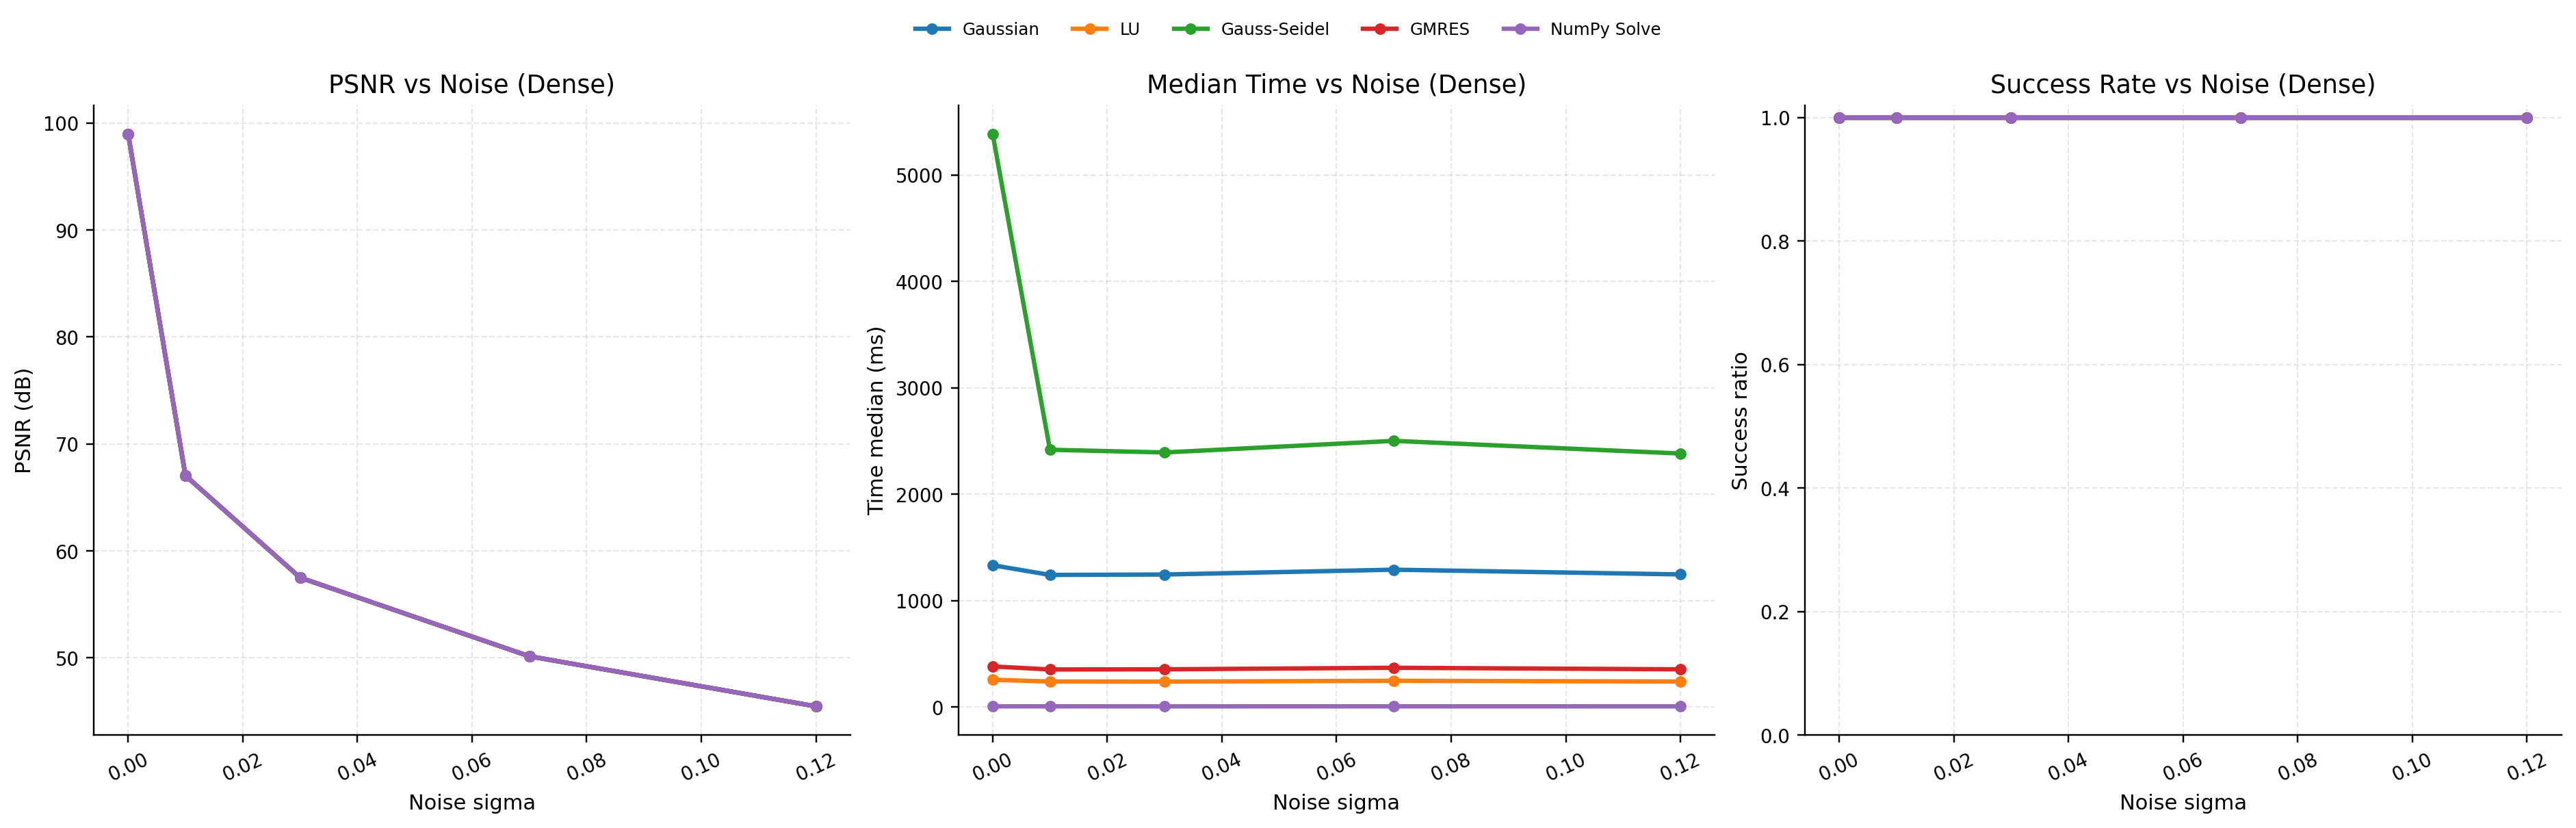
\includegraphics[width=0.8\textwidth]{out/figures/metrics_dense.png}
    \caption{Dense-key trends across noise for the compared solvers.}
    \caption*{This plot shows how reconstruction quality changes as noise increases when the key matrix is dense. Curves that stay higher and flatter indicate solvers that are more robust to noise, while steeper declines suggest greater sensitivity. The spacing between lines makes it easy to see which solver holds up best as corruption grows.}
\end{figure}

\begin{figure}[H]
    \centering
    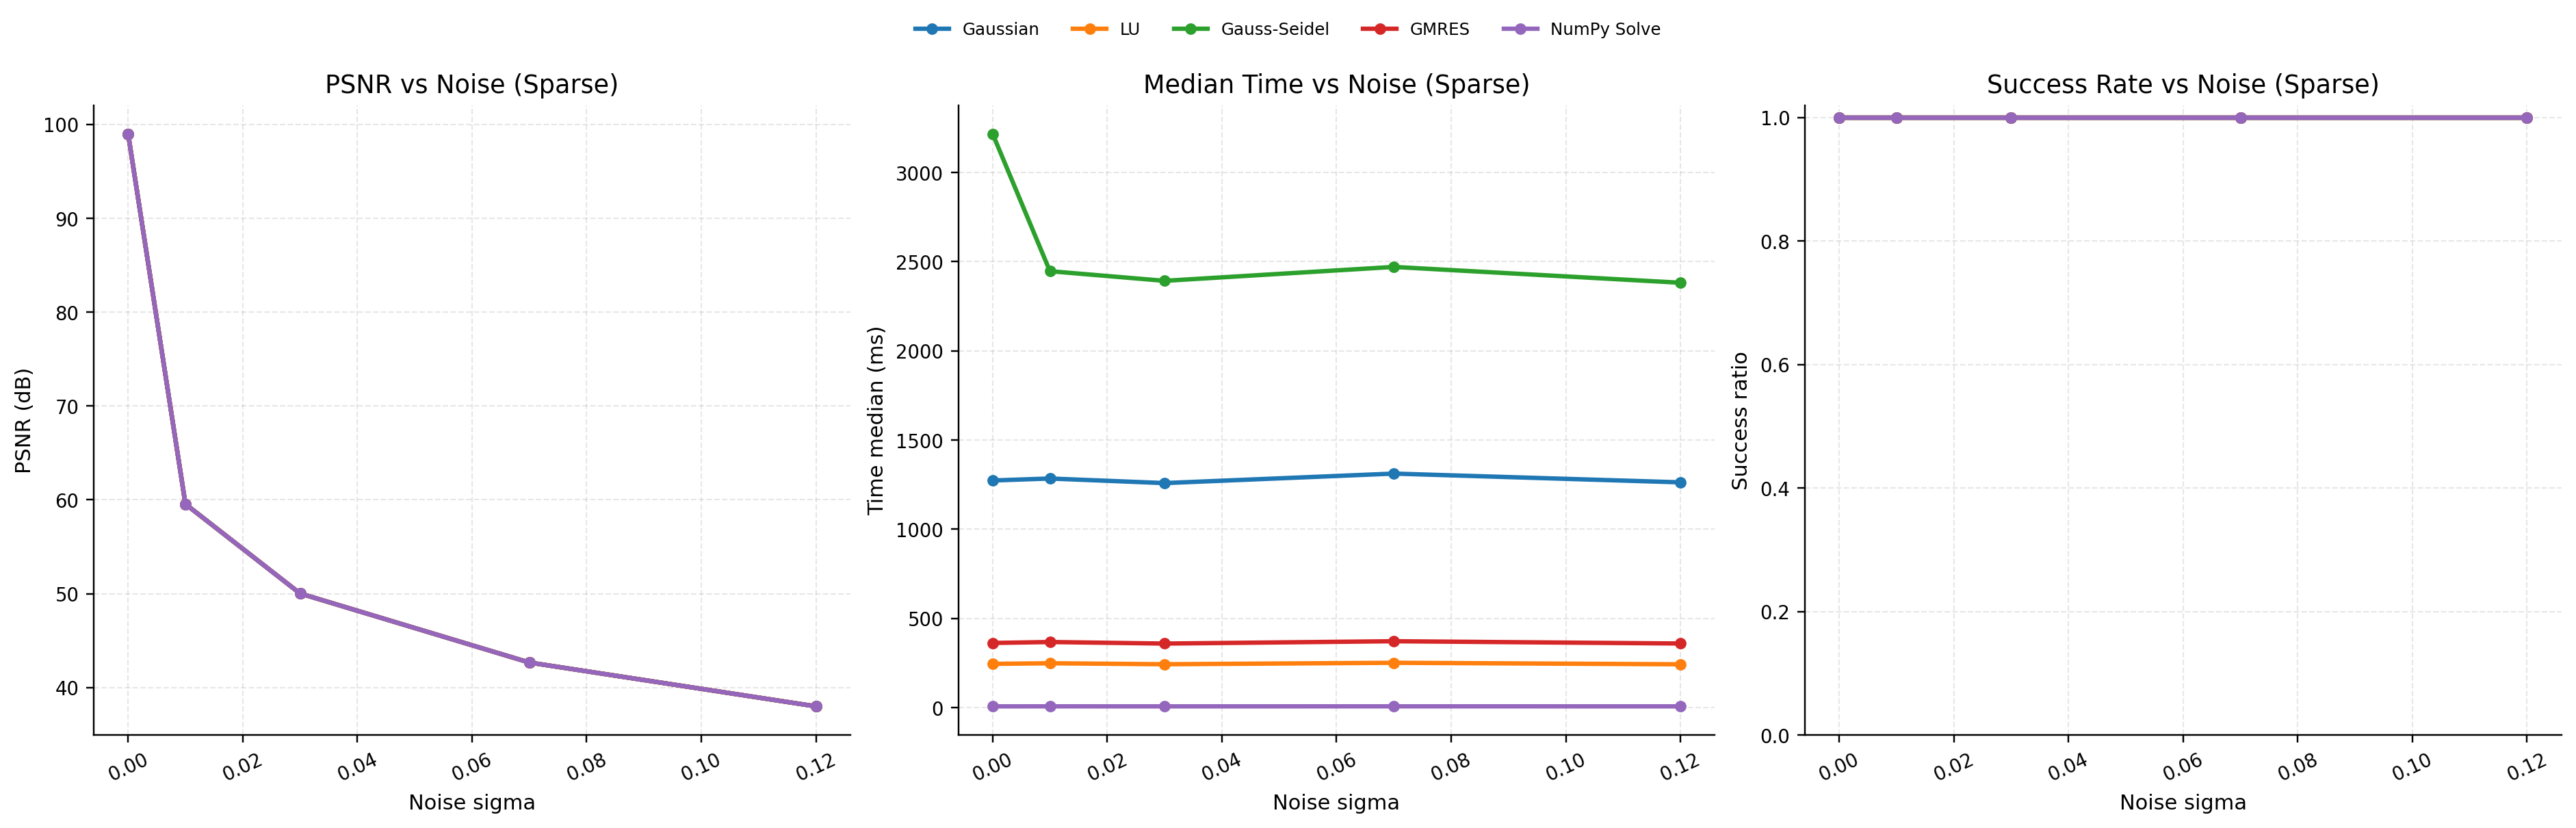
\includegraphics[width=0.8\textwidth]{out/figures/metrics_sparse.png}
    \caption{Sparse-key trends across noise for the compared solvers.}
    \caption*{This plot shows how reconstruction quality changes with noise when the key matrix is sparse. It helps the reader see whether sparsity makes the solvers degrade faster or more slowly compared with the dense case. Curves that stay higher indicate better robustness under the sparse structure.}
\end{figure}

\begin{figure}[H]
    \centering
    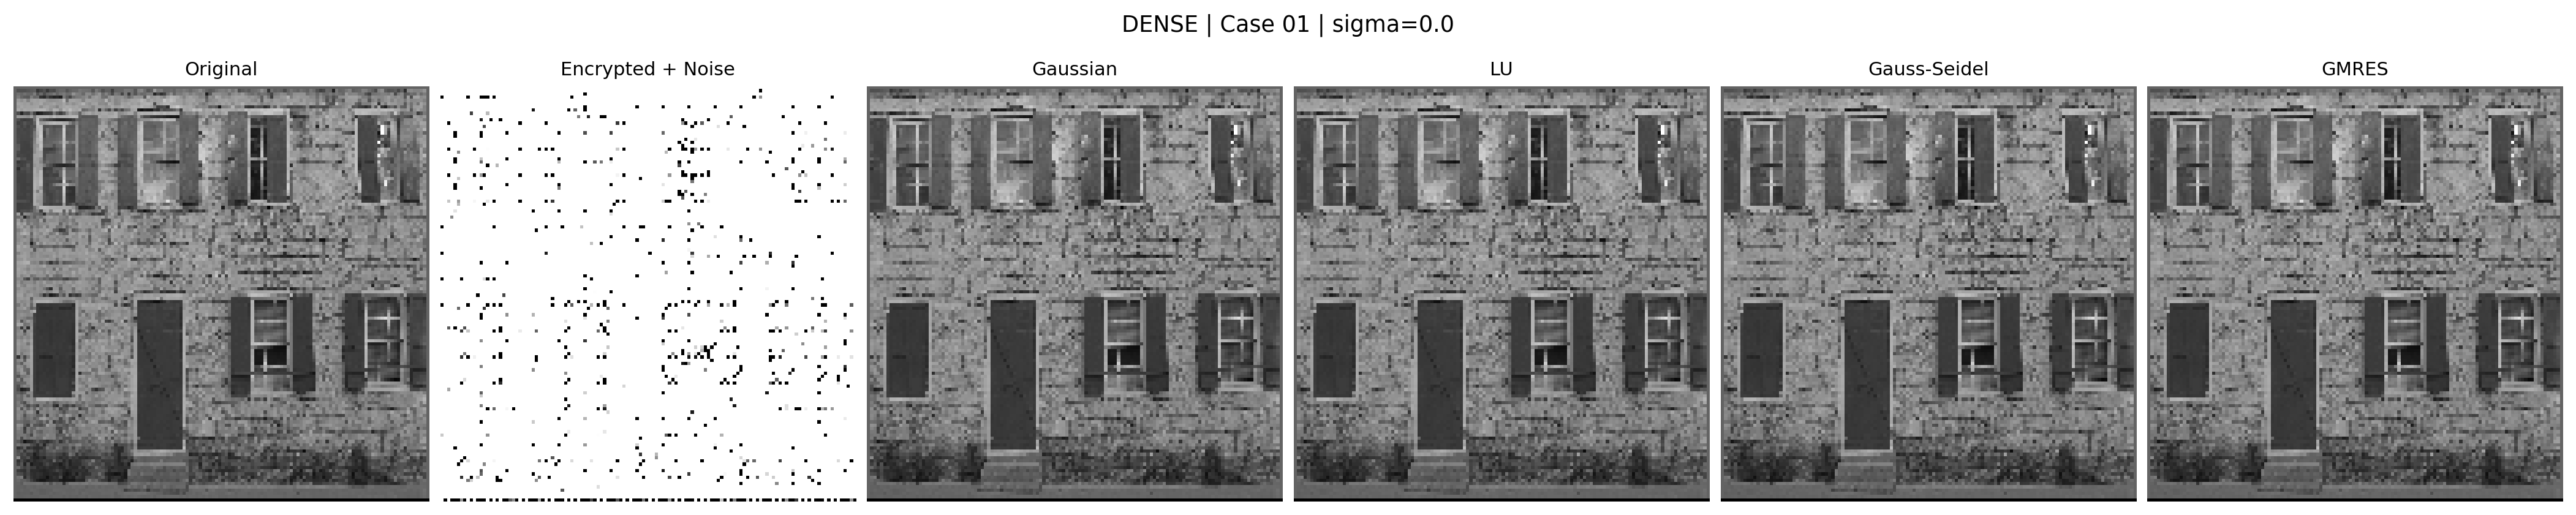
\includegraphics[width=0.9\textwidth]{out/figures/wall_01.png}
    \caption{Representative wall of decryption showing the original image, the encrypted-noisy image, and the recovered outputs from Gaussian, LU, Gauss-Seidel, and GMRES.}
    \caption*{The wall-of-decryption panel gives a side-by-side visual check of solver quality. Reconstructions that look closest to the original indicate better recovery, while visible artifacts show where noise and solver choice begins to break the image structure.}
\end{figure}

\begin{figure}[H]
    \centering
    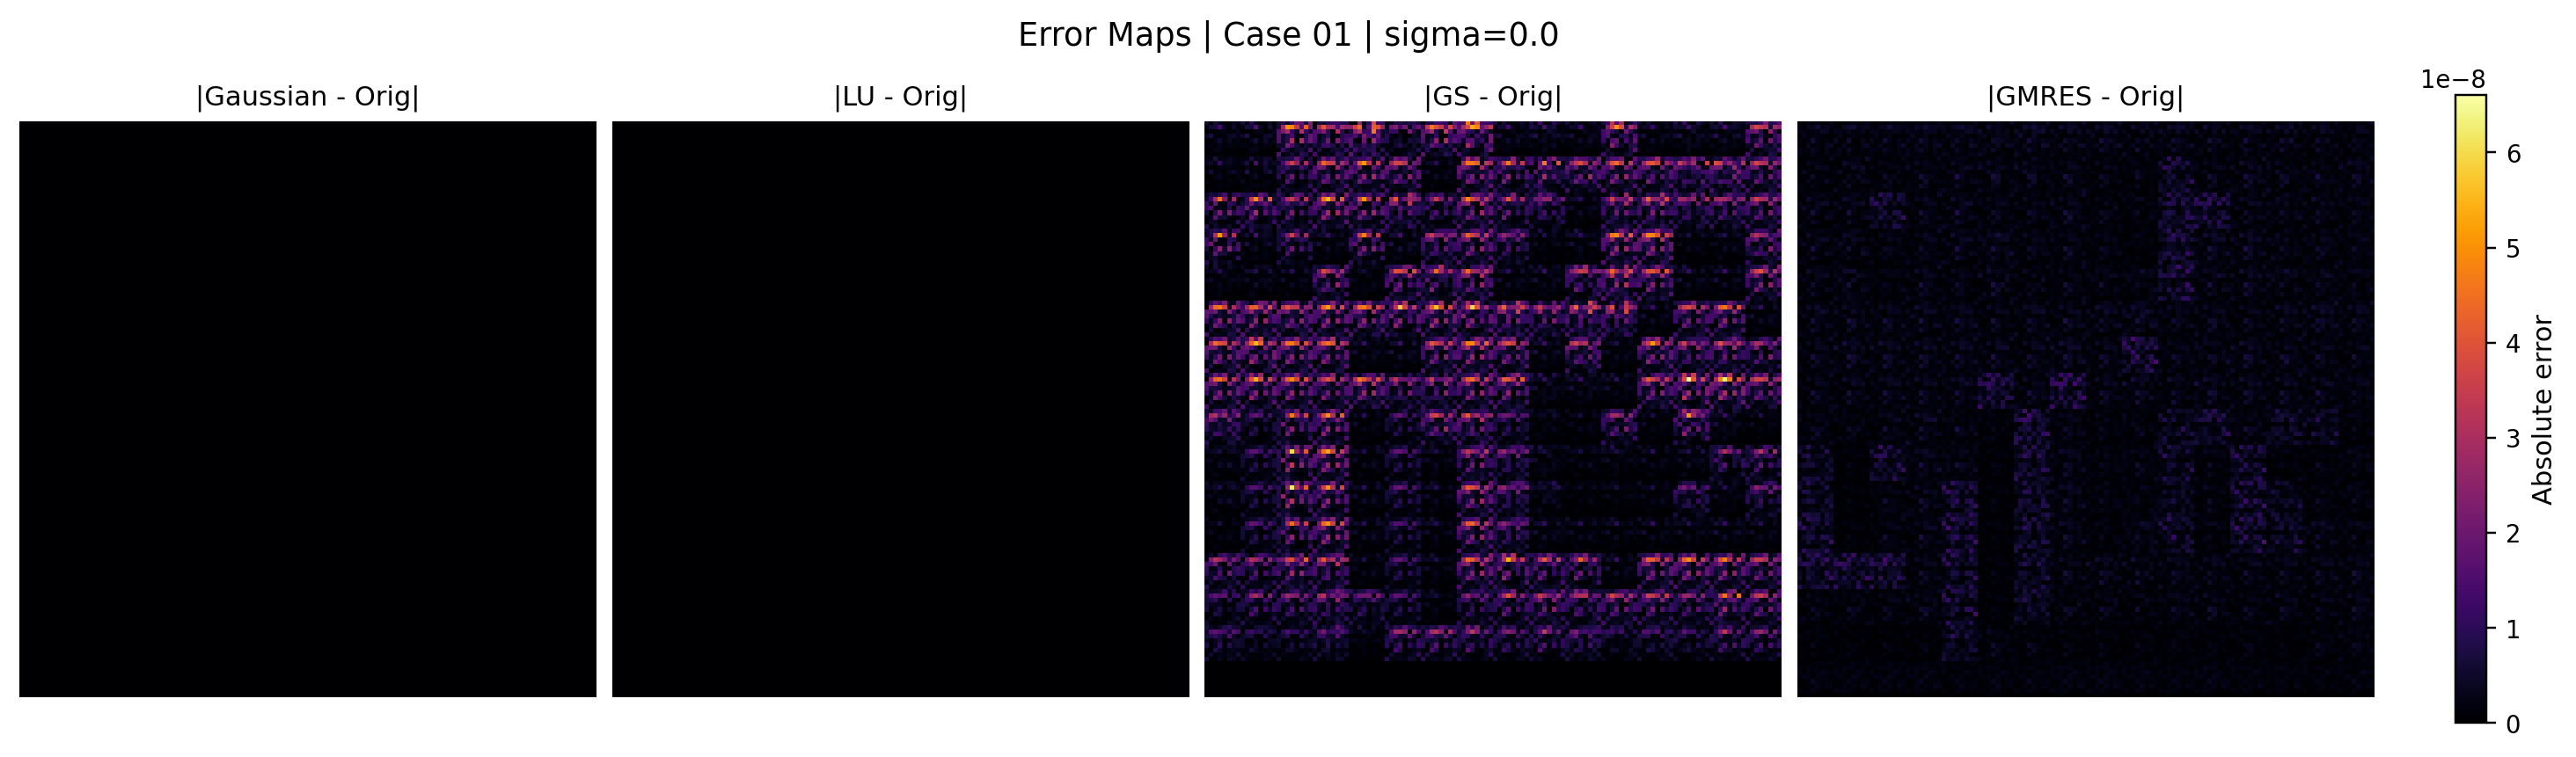
\includegraphics[width=0.9\textwidth]{out/figures/wall_err_01.png}
    \caption{Representative absolute-error maps for the first wall example.}
    \caption*{The error maps show where reconstruction deviates most from the original. Brighter regions mark larger errors, which helps the reader see whether mistakes cluster around edges, textures, or smooth areas.}
\end{figure}

\begin{figure}[H]
    \centering
    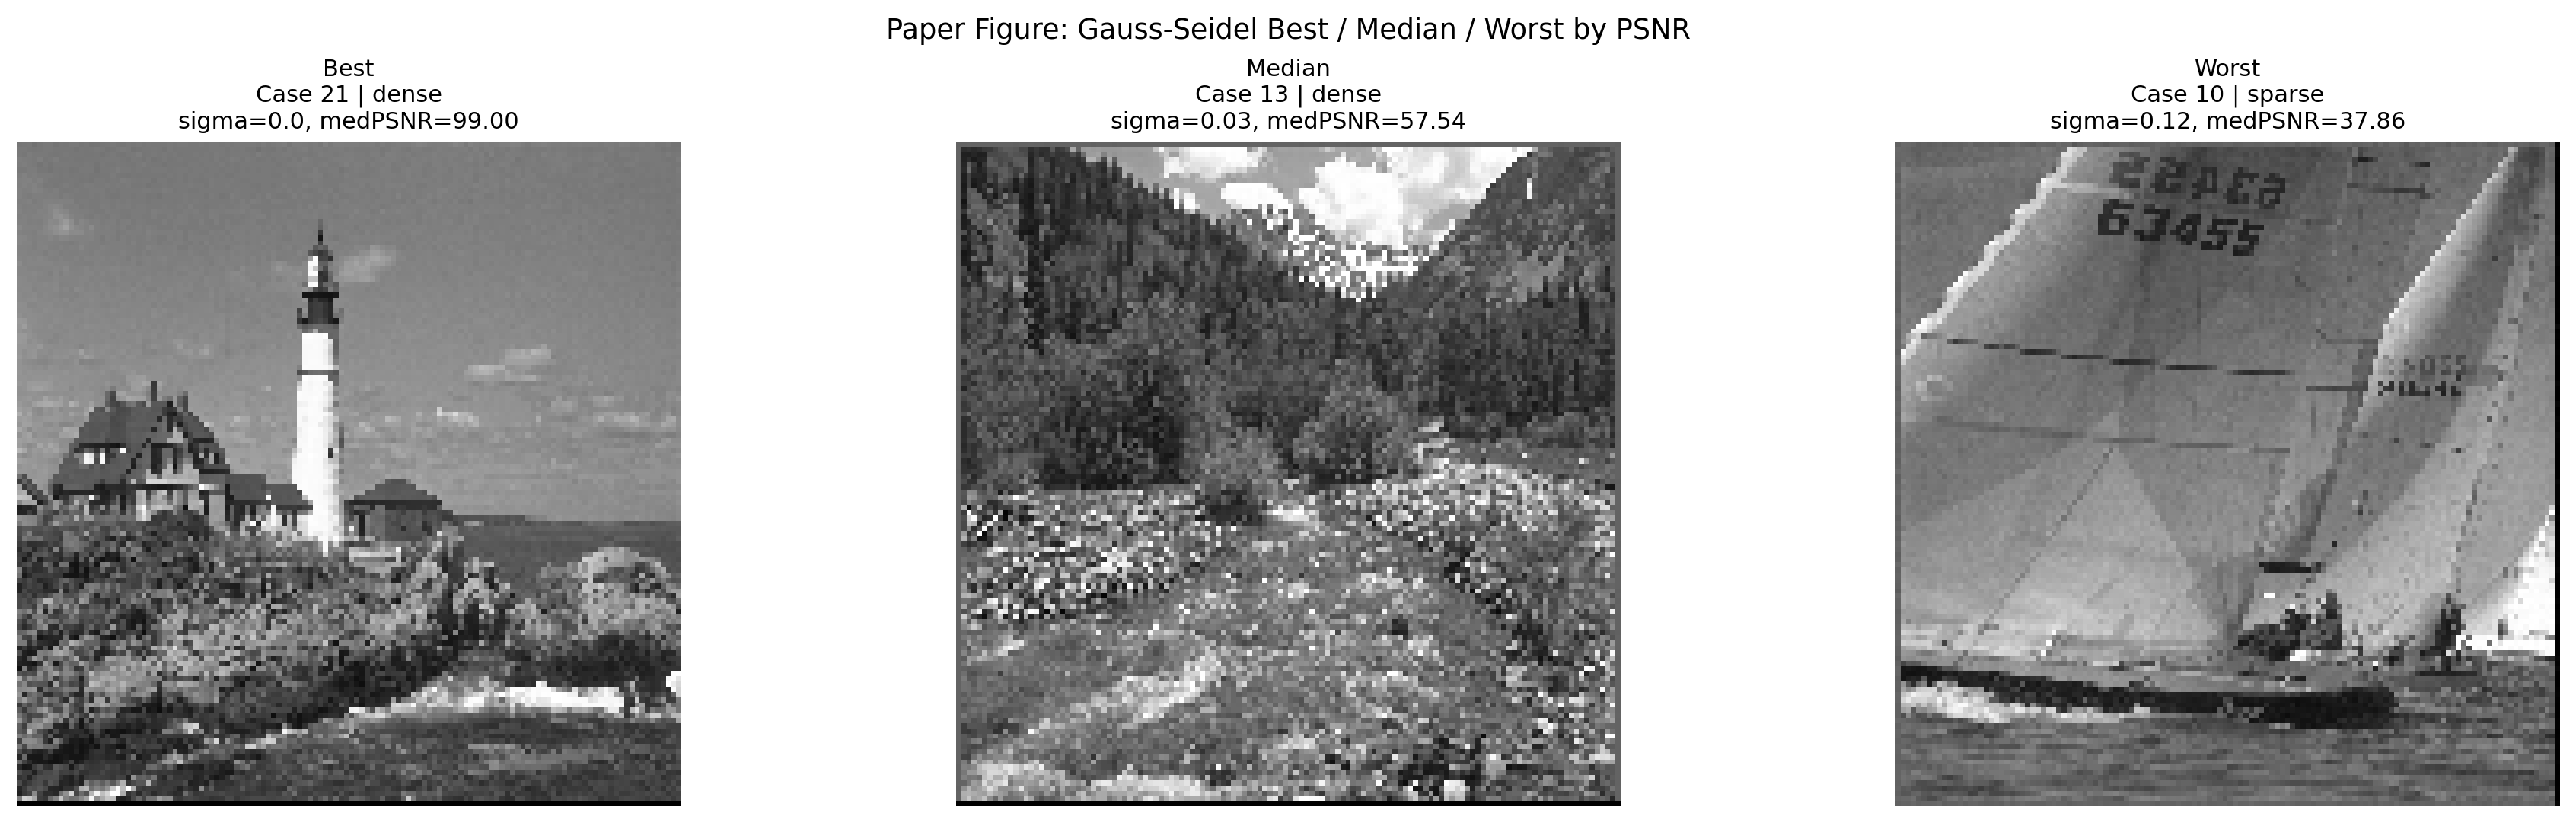
\includegraphics[width=0.9\textwidth]{out/figures/paper_triptych.png}
    \caption{Best, median, and worst Gauss-Seidel reconstruction examples by PSNR.}
    \caption*{The triptych summarizes variability within Gauss-Seidel by showing best, typical, and worst outcomes. It makes the range of expected quality easy to grasp without scanning all individual cases. It gives a quick visual sense of how much quality can vary for this solver, from strong recovery to visibly degraded output. The reader can see not just the average case, but also the range of outcomes Gauss-Seidel can produce under the same experimental setup.}
\end{figure}

\begin{figure}[H]
    \centering
    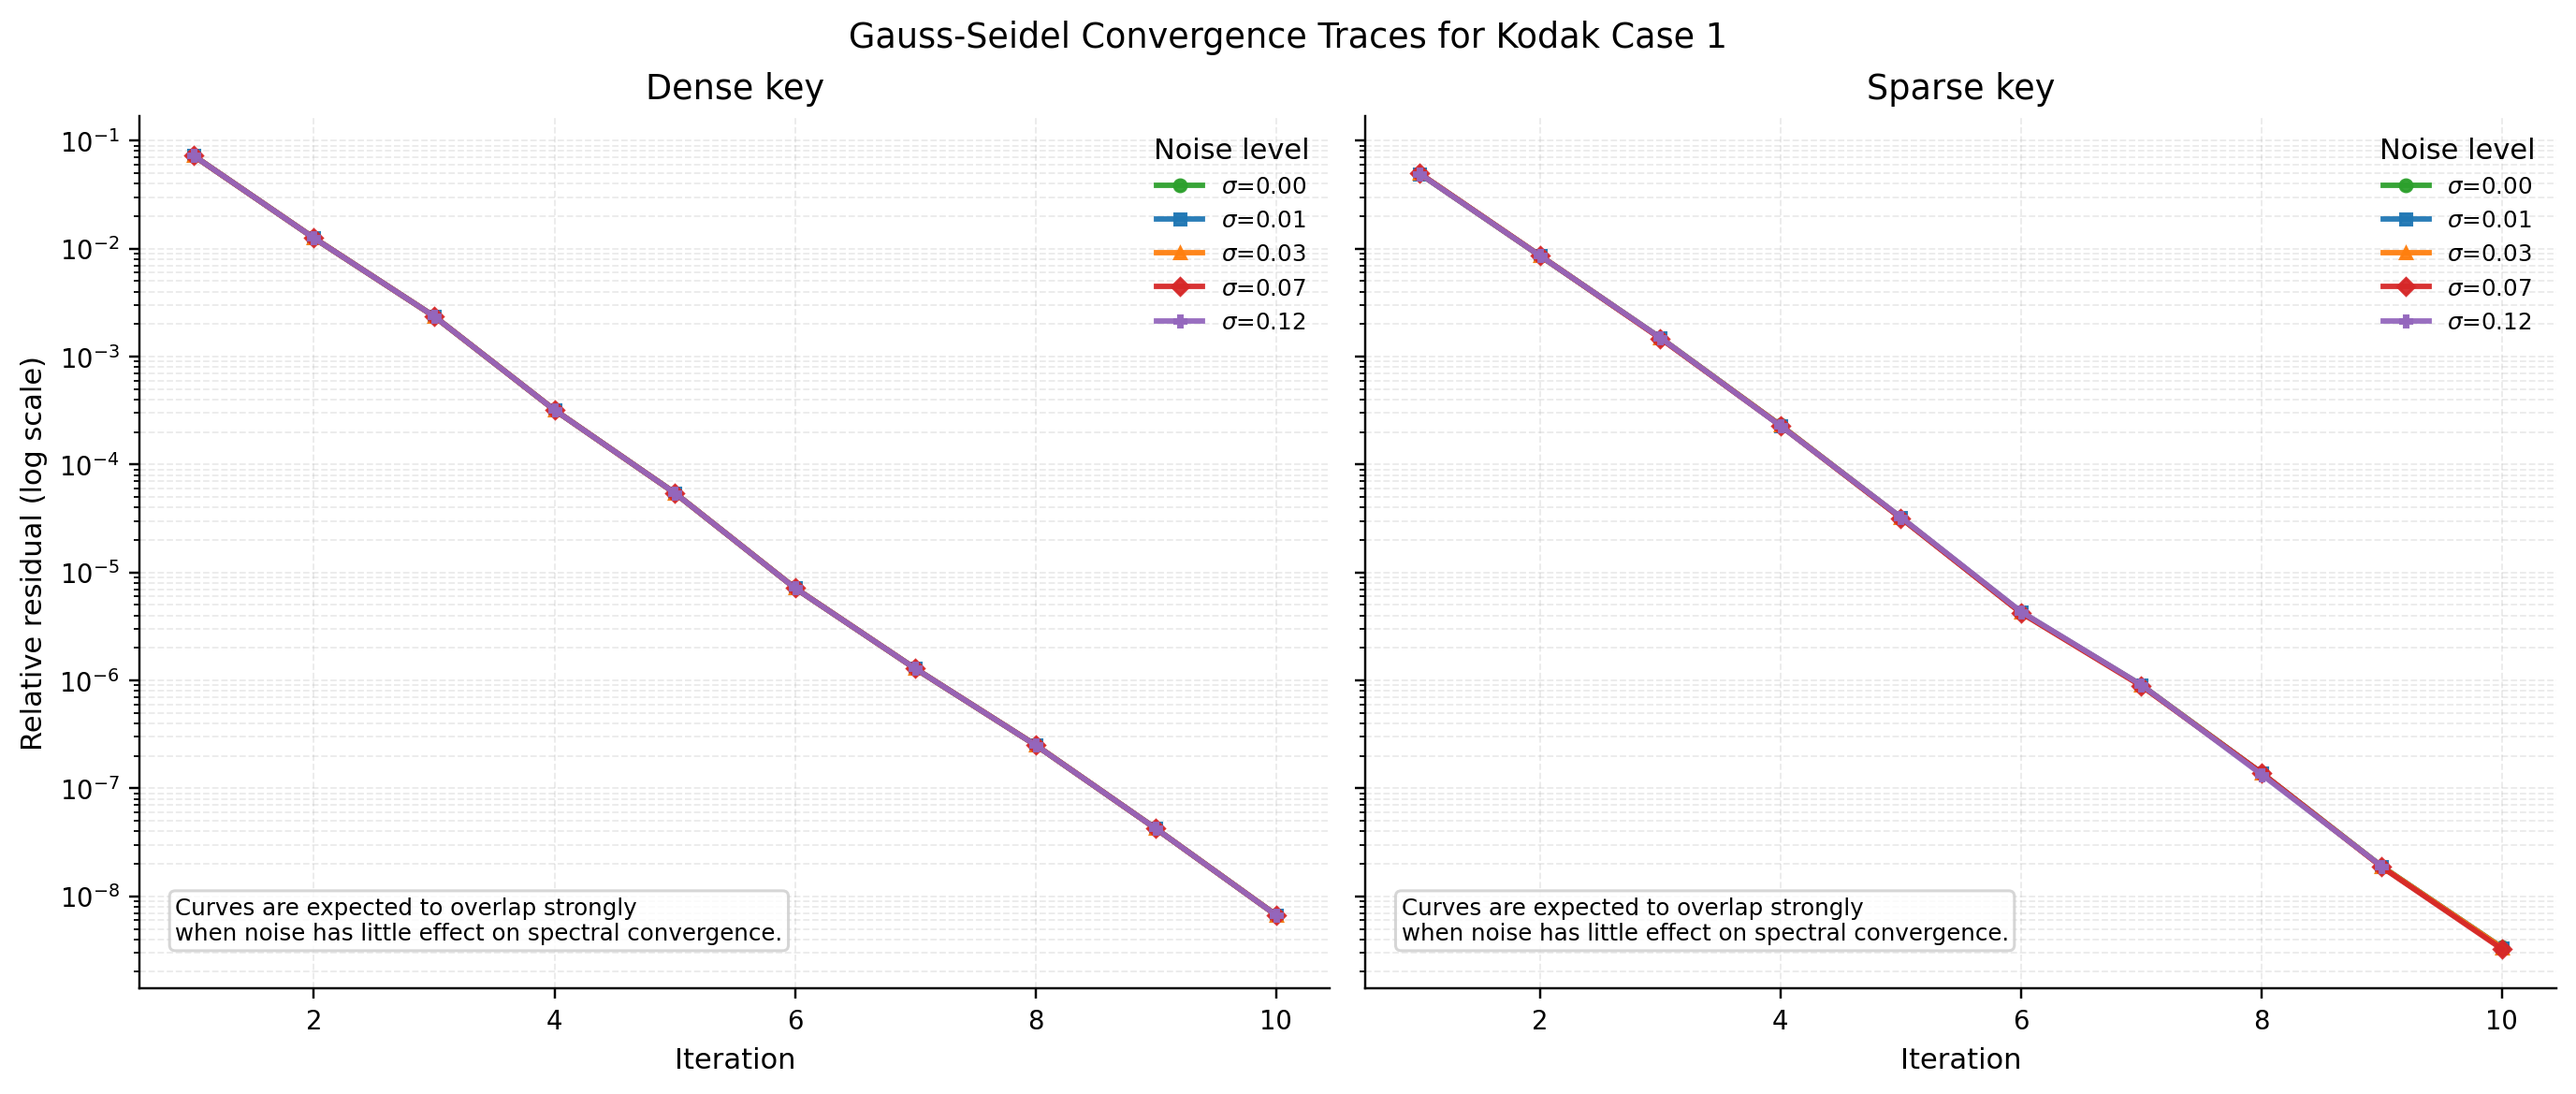
\includegraphics[width=0.8\textwidth]{out/figures/gs_convergence_traces.png}
    \caption{Gauss-Seidel convergence traces for the first Kodak case, split by dense and sparse keys.}
    \caption*{This figure shows how fast Gauss-Seidel reduces its residual over iterations for the first Kodak image. Steeper drops mean faster stabilization, while flatter curves mean slower progress. The dense versus sparse split helps the reader see how matrix structure affects convergence speed and stability.}
\end{figure}

\subsection{Results Highlights} 

First, LU is the speed leader. Averaged over all noise levels, its median solve time is about 244.71 ms for dense keys and 246.03 ms for sparse keys, well ahead of Gaussian Elimination, GMRES, and Gauss-Seidel. 

Second, GMRES shows the most reliable convergence among the iterative methods. Its full-convergence rate is 1.0 for both dense and sparse matrices across all tested noise levels, while Gauss-Seidel drops to an overall full-convergence rate of 0.833 because some zero-noise cases reach the iteration ceiling before satisfying the strict stopping rule. All methods still achieve a solve-success rate of 1.0, so the practical difference is convergence reliability rather than outright failure.

\section{Discussion} 

The researcher interprets the results in terms of real-world use, where encrypted images must be recovered even when the data are imperfect. Hospitals transmit scans across networks, satellites downlink compressed imagery, and secure media pipelines store or stream files that may pick up noise. In each case, small numerical errors in the ciphertext can turn into visible artifacts after decryption. The study provides a practical way to choose solvers that reduce that risk while balancing speed and stability.

The tables show that reconstruction quality (PSNR) is essentially the same across solvers for a given matrix type in the summarized setting. This means the meaningful differences are runtime and convergence reliability. LU remains the speed leader when the same key matrix is reused across many blocks, because the factorization cost is paid once and the repeated solves are cheap. GMRES delivers the most consistent full convergence under noise, while Gauss-Seidel can still recover blocks but occasionally stops at the iteration cap before meeting the strict convergence test.

Matrix structure also matters. Even when dense and sparse keys yield similar PSNR, they can lead to different runtime profiles and convergence behavior. This is important for deployment choices: if speed is the priority and the key is reused, LU is a strong default; if robustness to noisy corruption is the priority, GMRES is safer; and if the goal is to study iterative behavior, Gauss-Seidel provides clear convergence traces.  

This work is a numerical analysis study of matrix-based decryption workflows, not a security proof of modern cryptographic primitives. The conclusions should be read as guidance about numerical robustness, solver stability, and reconstruction quality rather than claims about cryptographic security.

\section{Conclusion}

\clearpage

\appendix
\section{Source Pseudocode}

\subsection{Gaussian Elimination with Partial Pivoting}


\begin{lstlisting}
INPUT: n, augmented matrix A = [a_ij], 1 <= i <= n, 1 <= j <= n+1
OUTPUT: x_1, ..., x_n or "no unique solution"

Step 1: For i = 1 to n set NROW(i) = i.

Step 2: For i = 1 to n-1 do:
  Step 3: Choose p with i <= p <= n such that
          |a(NROW(p), i)| = max_{i <= j <= n} |a(NROW(j), i)|.
  Step 4: If a(NROW(p), i) = 0, stop with "no unique solution".
  Step 5: If NROW(i) != NROW(p), interchange NROW(i) and NROW(p).
  Step 6: For j = i+1 to n do:
    Step 7: Set m(NROW(j), i) = a(NROW(j), i) / a(NROW(i), i).
    Step 8: Apply
            E_{NROW(j)} - m(NROW(j), i) E_{NROW(i)} -> E_{NROW(j)}.

Step 9:  If a(NROW(n), n) = 0, stop with "no unique solution".
Step 10: Set x_n = a(NROW(n), n+1) / a(NROW(n), n).
Step 11: For i = n-1 down to 1 set
         x_i = (a(NROW(i), n+1) - sum_{j=i+1}^{n} a(NROW(i), j) x_j)
               / a(NROW(i), i).
Step 12: Output x_1, ..., x_n.
\end{lstlisting}

\subsection{LU Decomposition (Doolittle Method)}


\begin{lstlisting}
Phase 1: LU decomposition in place
for k = 1 to n-1
  for i = k+1 to n
    a(i, k) = a(i, k) / a(k, k)
    for j = k+1 to n
      a(i, j) = a(i, j) - a(i, k) * a(k, j)
    end
  end
end

Phase 2: Forward substitution, solve L d = b
x(1) = b(1)
for i = 2 to n
  s = 0
  for j = 1 to i-1
    s = s + a(i, j) * x(j)
  end
  x(i) = b(i) - s
end

Phase 3: Back substitution, solve U x = d
x(n) = x(n) / a(n, n)
for i = n-1 down to 1
  s = 0
  for j = i+1 to n
    s = s + a(i, j) * x(j)
  end
  x(i) = (x(i) - s) / a(i, i)
end
\end{lstlisting}

\subsection{Gauss-Seidel with Relaxation (SOR)}


\begin{lstlisting}
SUBROUTINE Gseid(a, b, n, x, imax, es, lambda)

Step 1: Normalization
for i = 1 to n
  dummy = a(i, i)
  for j = 1 to n
    a(i, j) = a(i, j) / dummy
  end
  b(i) = b(i) / dummy
end

Step 2: Initial guess
for i = 1 to n
  sum = b(i)
  for j = 1 to n
    if i != j then
      sum = sum - a(i, j) * x(j)
    end
  end
  x(i) = sum
end

Step 3: Iterative refinement
iter = 1
do
  sentinel = 1
  for i = 1 to n
    old = x(i)
    sum = b(i)
    for j = 1 to n
      if i != j then
        sum = sum - a(i, j) * x(j)
      end
    end
    x(i) = lambda * sum + (1 - lambda) * old
    if sentinel == 1 and x(i) != 0 then
      ea = abs((x(i) - old) / x(i)) * 100
      if ea > es then
        sentinel = 0
      end
    end
  end
  iter = iter + 1
  if sentinel == 1 or iter > imax then
    exit
  end
end
\end{lstlisting}

\subsection{GMRES Hybrid}


\begin{lstlisting}
INPUT: key matrix A, encrypted block b, tolerance epsilon, cost factor delta
OUTPUT: decrypted image block x

Phase I: GMRES acquisition
1. Initialize x_0 and compute r_0 = b - A x_0.
2. While nu + 3 + delta < (1 + delta) (log epsilon / log tau - 1) do:
   a. Perform an Arnoldi step to expand the Krylov subspace.
   b. Update the residual reduction factor tau = ||r_nu|| / ||r_0||.
   c. Store coefficients of the implicit residual polynomial p_nu(z).

Phase II: Stabilized Richardson iteration
3. Compute roots zeta_1, ..., zeta_nu of p_nu(z).
4. Order the roots with a weighted Leja sequence for numerical stability.
5. While ||r_n|| > epsilon do:
   a. Update x_j = x_{j-1} + r_{j-1} / zeta_j.
   b. If the convergence rate falls below sqrt(tau), restart Phase I.
6. Return x.
\end{lstlisting}

\section{Complete Kodak Reconstruction Walls}

\ifincludeappendixwalls
\subsection{Reconstruction Walls}
\foreach \idx in {01,02,03,04,05,06,07,08,09,10,11,12,13,14,15,16,17,18,19,20,21,22,23,24}{%
\artifactfigure{out/figures/wall_\idx.png}{0.98}{Wall of decryption for Kodak case \idx.}%
}

\subsection{Absolute Error Maps}
\foreach \idx in {01,02,03,04,05,06,07,08,09,10,11,12,13,14,15,16,17,18,19,20,21,22,23,24}{%
\artifactfigure{out/figures/wall_err_\idx.png}{0.92}{Absolute-error maps for Kodak case \idx.}%
}
\else
\paragraph{Appendix note} The full reconstruction walls and error maps are available in \texttt{appendix\_walls.tex}. Enable them by setting \texttt{\string\includeappendixwallstrue} in the preamble.
\fi

\clearpage

\FloatBarrier

{\sloppy
\begin{thebibliography}{99}
\raggedright

\bibitem{alghamdi-munir-2024}
Alghamdi, Y., \& Munir, A. (2024). Image encryption algorithms: A survey of design and evaluation metrics. \textit{Journal of Cybersecurity and Privacy, 4}(1), 126--152. \url{https://doi.org/10.3390/jcp4010007}

\bibitem{burden-faires-2015}
Burden, R. L., \& Faires, J. D. (2015). \textit{Numerical analysis} (10th ed.). Cengage Learning.

\bibitem{chapra-canale-2010}
Chapra, S. C., \& Canale, R. P. (2010). \textit{Numerical methods for engineers} (6th ed.). McGraw-Hill.

\bibitem{kodak-lossless}
Eastman Kodak Company. (1999). \textit{Kodak lossless true color image suite}. \url{https://r0k.us/graphics/kodak/kodak/}

\bibitem{frankel-1950}
Frankel, S. P. (1950). Convergence rates of iterative treatments of partial differential equations. \textit{Mathematics of Computation, 4}, 65--75.

\bibitem{golub-vanloan-2013}
Golub, G. H., \& Van Loan, C. F. (2013). \textit{Matrix computations} (4th ed.). Johns Hopkins University Press.

\bibitem{gonzalez-woods-2018}
Gonzalez, R. C., \& Woods, R. E. (2018). \textit{Digital image processing} (4th ed.). Pearson.

\bibitem{lu-notes}
Kiruba, R. (2014). \textit{LU decomposition notes} (University of Cambridge supporting notes).
\newline\url{https://www.cl.cam.ac.uk/teaching/1314/NumMethods/supporting/mcmaster-kiruba-ludecomp.pdf}

\bibitem{nachtigal-gmres-1992}
Nachtigal, N. M., Reichel, L., \& Trefethen, L. N. (1992). A hybrid GMRES algorithm for nonsymmetric linear systems. \textit{SIAM Journal on Matrix Analysis and Applications, 13}(3), 796--825. \url{https://doi.org/10.1137/0613050}

\bibitem{noura-2017}
Noura, H., Sleem, L., \& Couturier, R. (2017). \textit{A revision of a new chaos-based image encryption system: Weaknesses and limitations} (arXiv preprint). \url{https://arxiv.org/abs/1701.08371}

\bibitem{saad-2003}
Saad, Y. (2003). \textit{Iterative methods for sparse linear systems} (2nd ed.). Society for Industrial and Applied Mathematics.

\bibitem{trefethen-bau-1997}
Trefethen, L. N., \& Bau, D., III. (1997). \textit{Numerical linear algebra}. SIAM. \url{https://doi.org/10.1137/1.9780898719574}

\bibitem{varga-1962}
Varga, R. S. (1962). \textit{Matrix iterative analysis}. Prentice-Hall.

\bibitem{young-1950}
Young, D. M. (1950). \textit{Iterative methods for solving partial difference equations of elliptic type} (Doctoral dissertation, Harvard University).

\end{thebibliography}
}

\end{document}
